


\documentclass[10pt, handout]{beamer}
\setbeamertemplate{navigation symbols}{}
\usefonttheme{serif} 
\usepackage{amsmath}
\usepackage{amssymb}
\usepackage{graphicx}
\usepackage{cite}
\usepackage{color} 
\usepackage{setspace}
\usepackage{hyperref}

\newcommand{\xx}{{\bf{x}}}

\begin{document}
\title{Machine Learning I Lecture VII:\\ Logistic Regression}   
\author{Jakob H Macke\\ Max Planck Institute for Biological Cybernetics\\ Bernstein Center for Computational Neuroscience} 
\date{\today} 

\frame{\titlepage} 

%\frame{\frametitle{Today: Back to basics of probability theory}} 


\frame{\frametitle{Plan for today}\tableofcontents} 

\section{Logistic Regression}

\frame{\frametitle{For the linear classification model, we assumed the class-conditional distributions to be Gaussian}
\begin{itemize}
\item We assumed $x| (t=1) \sim \mathcal{N}(\mu_+, \Sigma_+)$ and $x| (t=-1) \sim \mathcal{N}(\mu_-, \Sigma_-)$, and two class-probabilities $P(t=1)$ and $P(t=-1)$.
\item \pause This is called an \alert{generative model}, as we have written down a full joint model over the data. 
\item \pause We saw that violations of the model assumption can lead to `bad' decision boundaries.
\end{itemize}
\begin{center}
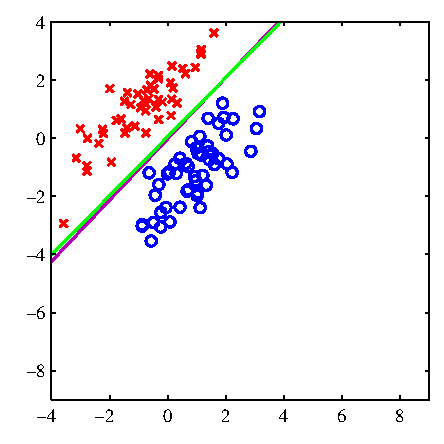
\includegraphics[width=.35\textwidth]{Figure44a.pdf}
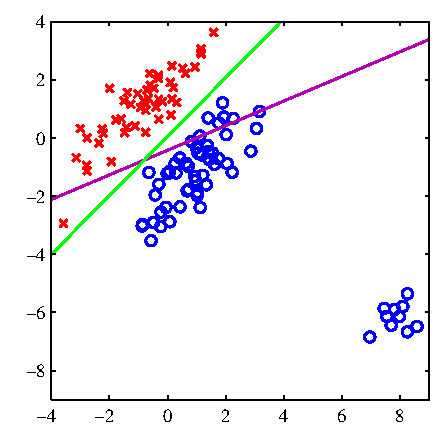
\includegraphics[width=.35\textwidth]{Figure44b.pdf}

\tiny Figures from Bishop PRML, 44a and b
\end{center}
} 

\frame{\frametitle{For regression, we assumed Gaussian outputs, but did not need assumptions about the distribution of inputs.}
\begin{itemize}
\item For linear regression, we conditioned on $x$, and assumed a Gaussian distribution over $t$: $t|x \sim \mathcal{N}(y(x), \gamma^2)$
\item \pause We maximized the conditional log-likelihood $L(\omega)=\sum_n \log p(t_n|x_n, \omega)$, i.e we assumed that the $x$ were given.
\item \pause Therefore, this approach to linear regression works for \alert{any} distribution over $x$.
\item $x$ is typically high-dimensional, so it is difficult to make appropriate distributional assumptions for it. 
\end{itemize}
\begin{center}
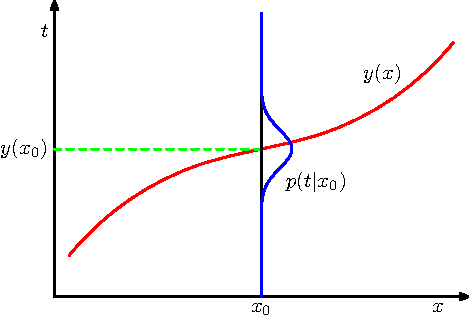
\includegraphics[width=.4\textwidth]{Figure128.pdf}

\tiny Figure Bishop PRLM 128
\end{center}
} 



\frame{\frametitle{We can define a discriminative model for classification by modelling the conditional class probabilities.}
\begin{itemize}
\item From the homework-exercise, we know that $P(t=1 | z(x))=\sigma(z(x))$ where $\sigma(z)=1/(1+\exp(-z))$ and $z(x)=
\omega^\top x+\omega_o$.
\item Notation is simpler if we use $0$ and $1$ as class labels, so we define $s_n=1$ as the label for the positive class, and $s_n=0$ als label for the negative class.
\item In other words, $s |x \sim \mbox{Bernoulli}(\sigma(y(x))$.
\item Also, we set $y_n=\sigma(z(x))$.
\item \pause The parameters of $z(x)=\omega^\top x+ \omega_o$ can be learned by maximizing the conditional log-likelihood $L(\omega)=\sum_n \log p(t_n|x_n, \omega)$ [on board]
\item \pause This is an \alert{discriminative} approach to classification, as we only model the labels, and not the inputs.
\item 
\pause Decision rule and function shape of $p(t|x)$ will be the same for the generative (`Linear Discriminant Analysis') and the discriminative model, but the parameters were obtained differently.
\end{itemize}
} 

\section{Maximum likelihood estimation of Logistic Regression}


\frame{\frametitle{Maximum likelihood estimation of Logistic Regression}
\begin{center}
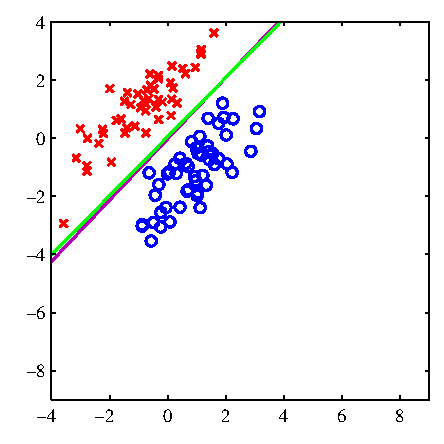
\includegraphics[width=.35\textwidth]{Figure44a.pdf}
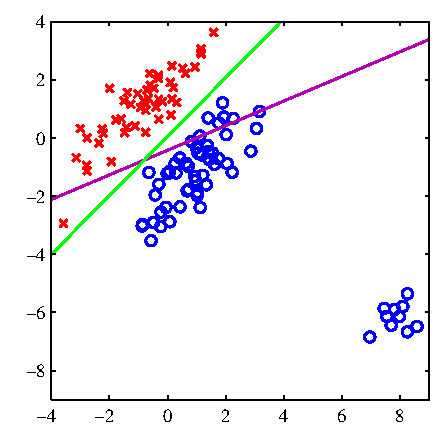
\includegraphics[width=.35\textwidth]{Figure44b.pdf}

\tiny Bishop PRML Figure 44 a and b
\end{center}
\begin{itemize}
\item This algorithm is called \alert{logistic regression}, and is a \emph{much} better algorithm than the algorithms we discussed last week.
\item Need to optimize log-likelihood numerically.
\item \pause People typically minimize the negative log-likelihood $\mathcal{L}$ rather than maximize the log-likelihood...
\item \pause To numerically minimize the negative log-likelihood, we need its gradient (and maybe its hessian) [on board]
\end{itemize}
}

\frame{\frametitle{The cost-function for logistic regression is convex.}
\begin{center}
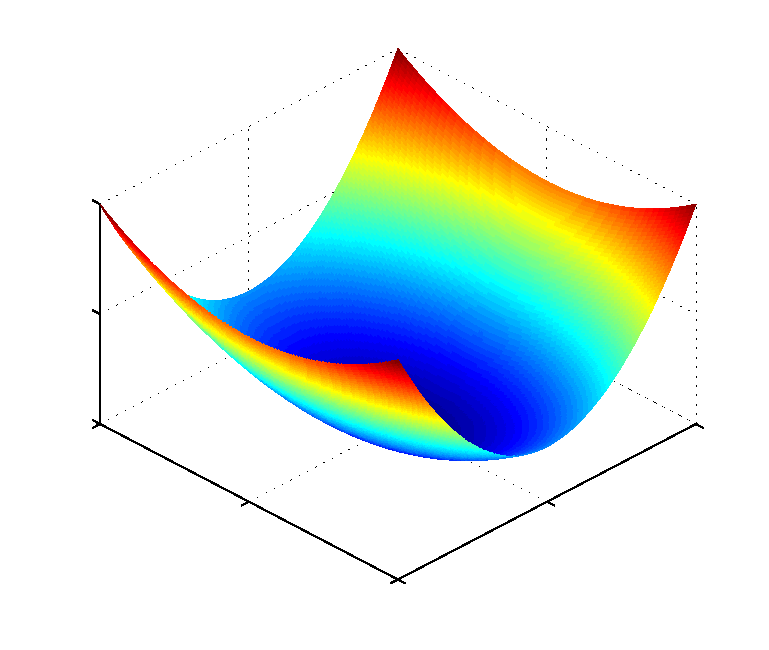
\includegraphics[width=.48\textwidth]{Convex.pdf}
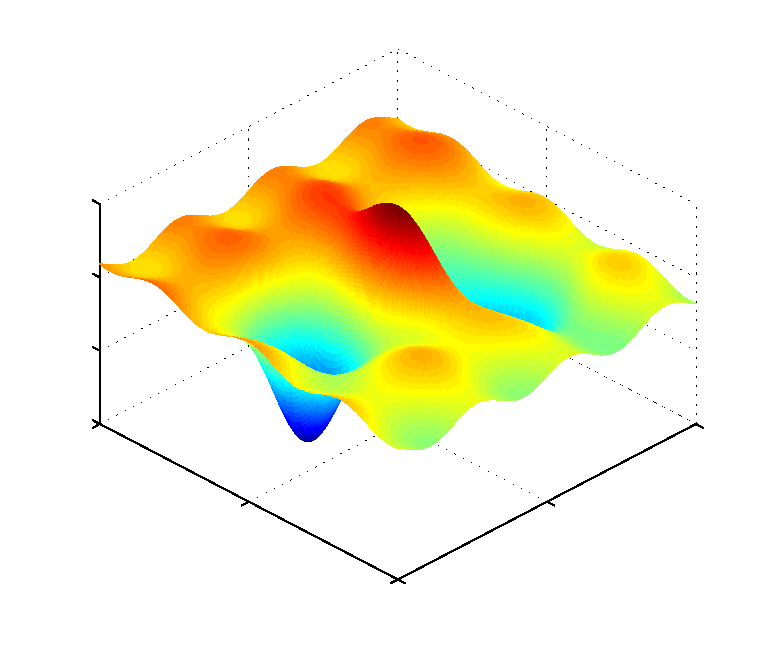
\includegraphics[width=.48\textwidth]{NotConvex.pdf}
\end{center}
\begin{itemize}
\item \pause Fact: The negative log-likelihood is \emph{convex} -- this makes life much more easier. 
\item \pause There are no local minima to get stuck in, and there is good optimization techniques for convex problems. 
\end{itemize}
}




\frame{\frametitle{\emph{Gradient descent} is a simple method for numerically minimizing a function.}
\begin{itemize}
\item The gradient $\nabla \mathcal{L}$ of a function points into the direction of steepest descent.
\item \pause Gradient descent: 'run down the gradient' $\omega_{new}=\omega_{old}-\alpha \nabla \mathcal{L}_\omega$, with learning rate $\alpha$.
\item \pause Slightly more sophisticated version: numerically optimize $\alpha$ for each step by doing a \emph{line search}.
\item \pause Convergence can be very slow if cost-function has `valleys'.
\end{itemize}
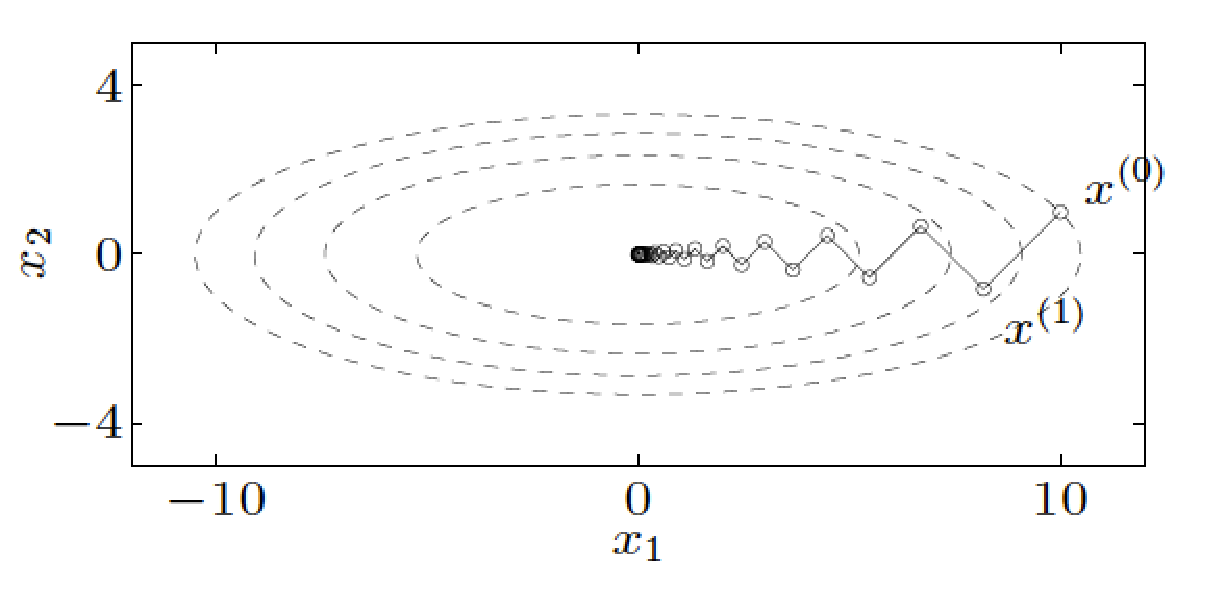
\includegraphics[width=.7\textwidth]{BoydGradientDescent}

\tiny Figure from Stephen Boyd, Convex Optimization
}

\frame{\frametitle{\emph{Iterative Least Squares:} Approximate by parabola, minimze, iterate.}
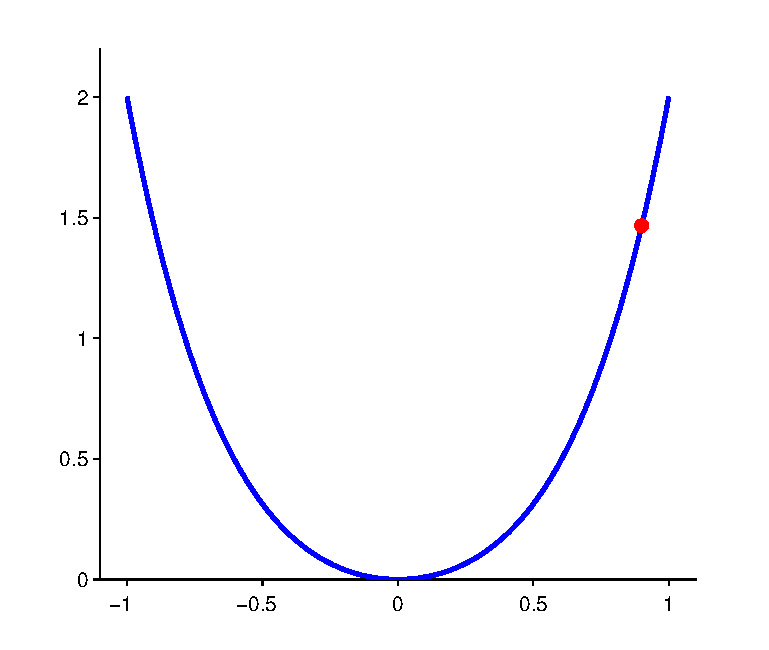
\includegraphics[width=.8\textwidth]{Newton0}
}

\frame{\frametitle{\emph{Iterative Least Squares:} Approximate by parabola, minimze, iterate.}
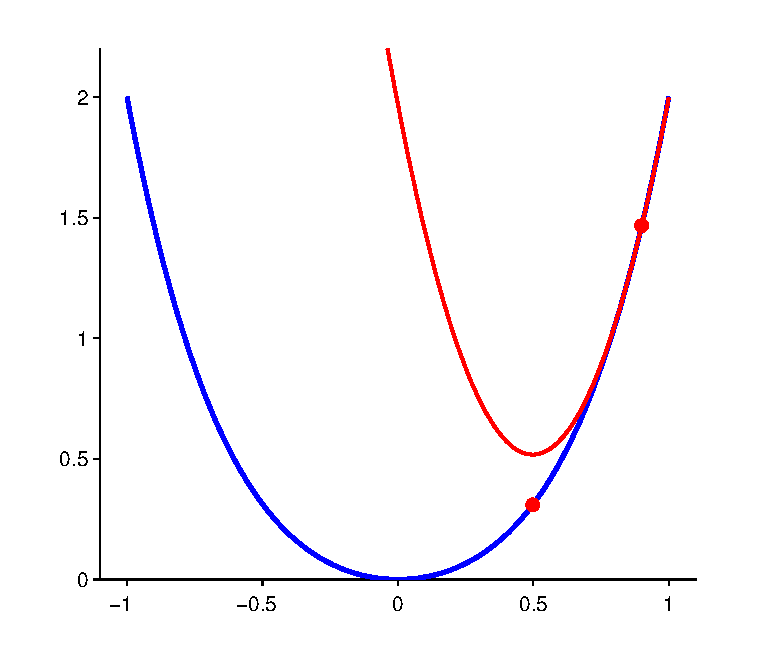
\includegraphics[width=.8\textwidth]{Newton1}
}

\frame{\frametitle{\emph{Iterative Least Squares:} Approximate by parabola, minimze, iterate.}
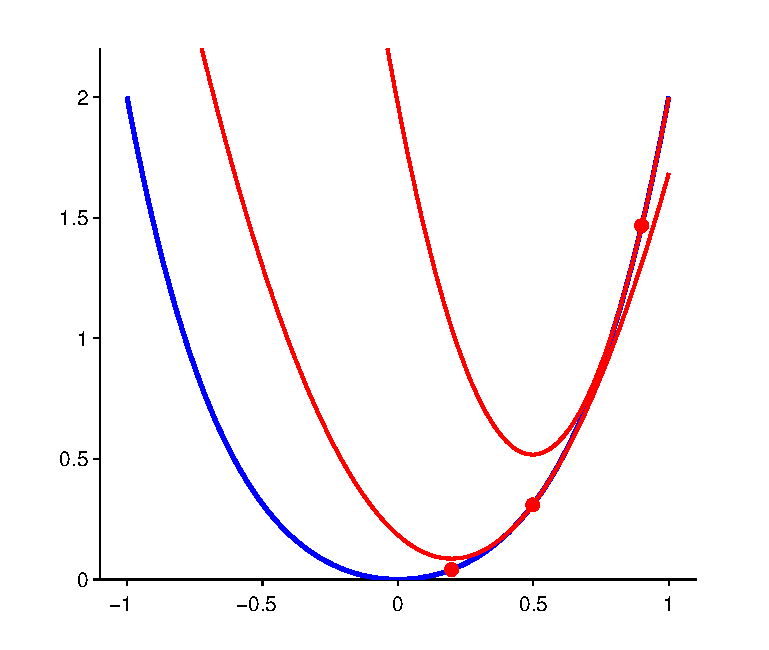
\includegraphics[width=.8\textwidth]{Newton2}
}


\frame{\frametitle{\emph{Iterative Least Squares:} Approximate by parabola, minimze, iterate.}
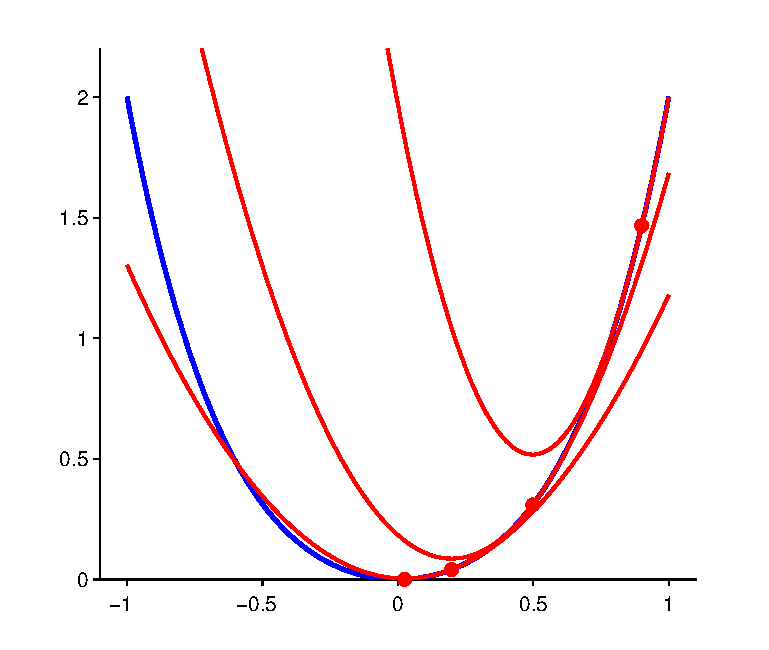
\includegraphics[width=.8\textwidth]{Newton3}
}

\frame{\frametitle{\emph{Iterative Least Squares:} Approximate by parabola, minimze, iterate.}
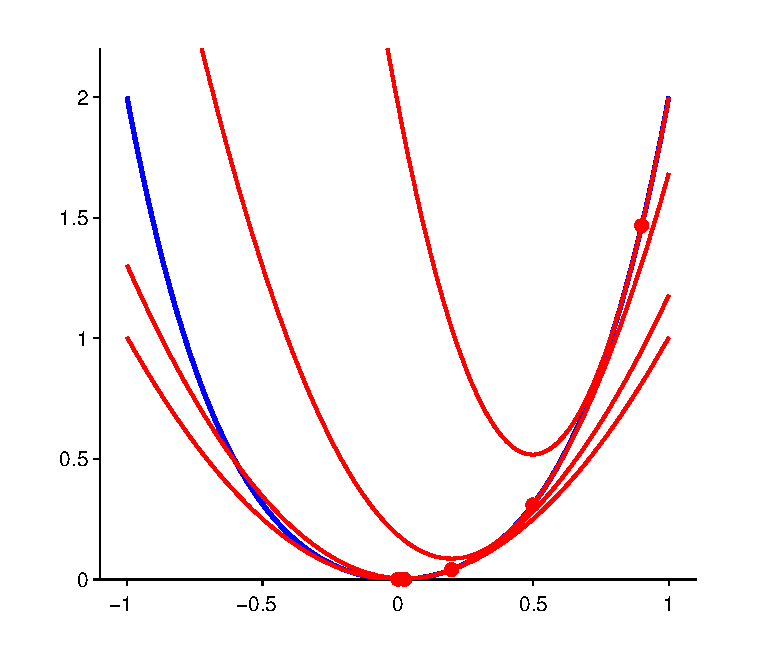
\includegraphics[width=.8\textwidth]{Newton4}
}
\frame{\frametitle{\emph{Iterative Least Squares:} Approximate by parabola, minimze, iterate.}
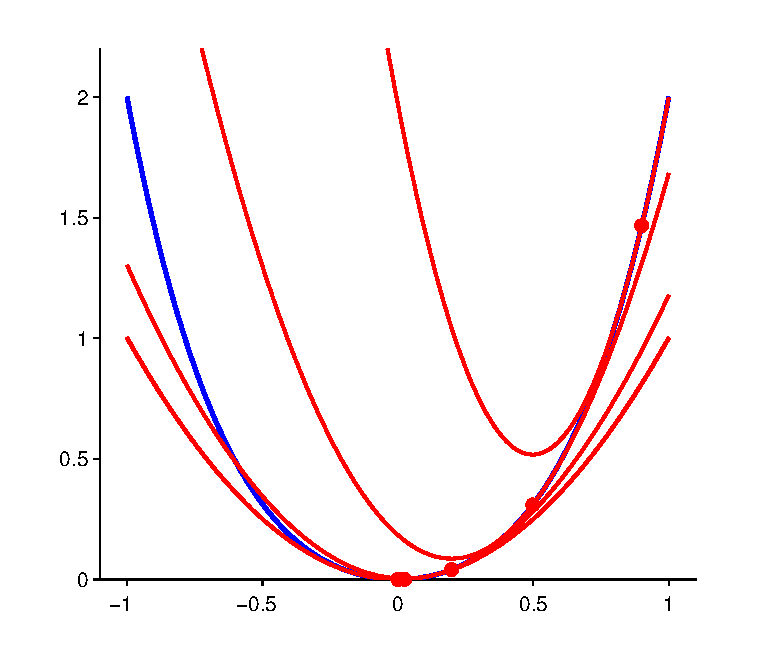
\includegraphics[width=.8\textwidth]{Newton5}
}
\frame{\frametitle{\emph{Iterative Least Squares:} Approximate by parabola, minimze, iterate.}
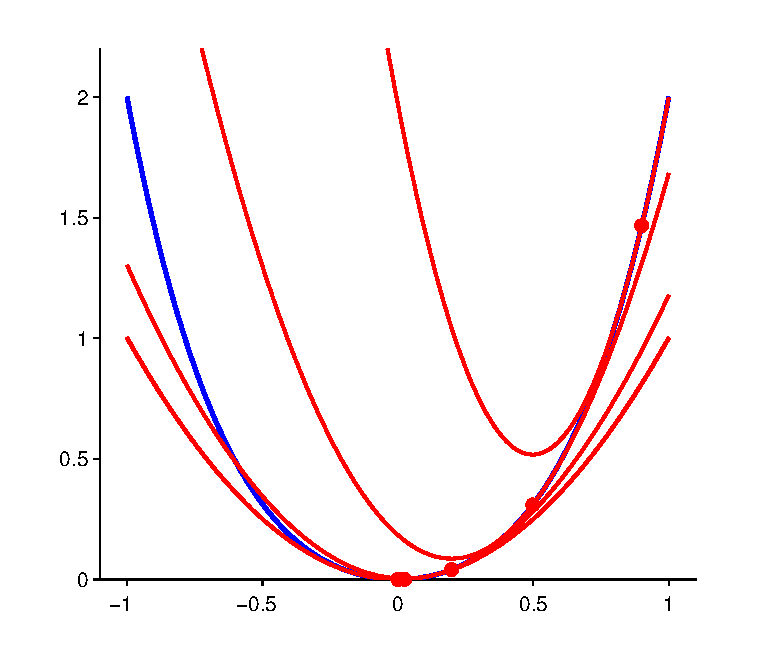
\includegraphics[width=.8\textwidth]{Newton6}
}



\frame{\frametitle{\emph{Iterative Least Squares} is a more efficient method for minimizing the cost-function}
\begin{itemize}
\item Newton-Raphson: $\omega_{new}=\omega_{old}-\alpha (\nabla \nabla \mathcal{L})^{-1}\nabla L_\omega$ 
\item Pre-multiplying the gradient by the inverse-hessian speeds up convergence `along valleys' (analogy with LDA)
 \item Motivation: For quadratic functions $F(x)=a+b^\top x+ x^\top B x$, Newton-Raphson finds the minimum in one iteration.
 \item In this contex, Newton-Raphson (with $\alpha=1$) is often called \alert{iterative least squares}.
 \item Note: Newtwn's method can be bad if problem is not convex, and can be slow if it is difficult to calculate/invert the Hessian. A large number of optimization algorithms exist which do not require the (complete) Hessian (quasi Newton/BFGS, etc..). 
% \item Any (reasonable) optimization algorithm requires the gradient.
\end{itemize}
}

\frame{\frametitle{Visualizing the cost-function of logistic regression}

[on board]

}

\section{Bayesian Logistic Regression: Approximating the posterior distribution}
\frame{\frametitle{Bayesian inference for this model does not have a closed form solution}
\begin{itemize}
\item Typically use Gaussian prior on $\omega$.
\item For linear regression, posterior distribution was Gaussian, with closed-form solutions for the mean and covariance.
\item For logistic regression, the posterior distribution is non-Gaussian.
\item \pause Popular approximation: Approximate posterior by a Gaussian
\begin{align}
p(\omega|D) \approx \mathcal{N}(\mu_{post}, \Sigma_{post})
\end{align}
\item \pause Different methods exist for finding `good' $\mu_{post}$ and $\Sigma_{post}$: Expectation Propagation (EP), Laplace Approximation, Variational Inference
\end{itemize}

}

\frame{\frametitle{The Laplace-Approximation is a simple Gaussian approximation to the posterior}
\begin{itemize}
\item \alert{Laplace approximation:} $\mu_{post}=\omega_{MAP}$, $\Sigma_{post}=\left(\nabla \nabla_\omega L   \right)^{-1}$. 
\item Take MAP as mean, and inverse hessian at MAP as covariance.
\item \pause Motivation: Curvature matching, Taylor-expansion [on board]
\item \pause Q: When will the Laplace approximation fail?
\end{itemize}
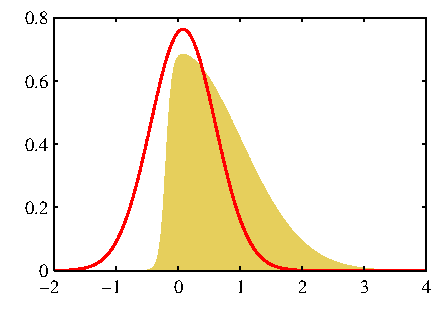
\includegraphics[width=.49\textwidth]{Figure414a.pdf}
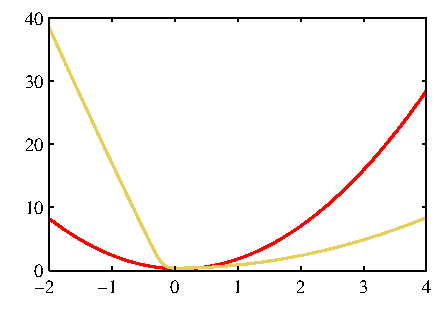
\includegraphics[width=.49\textwidth]{Figure414b.pdf}

\tiny Figure from Bishop PRML Figures 414a and b
}

\frame{\frametitle{The posterior distribution can be used to calculate the predictive distribution and to optimze hyper-parameters}
[on board]

}


%\section{LR's popular little brother-- support vector machines}

%\section{The exam}



\frame{\frametitle{One last bit of business: The exam}

\begin{itemize}
\item Next Friday, 2pm \emph{sharp}.
\item You will have 90 minutes.
\item You are allowed to use a pen or other writing utensils and your brain, no other tools/materials/books/notes will be allowed.
\item All mobiles phones need to be switched off.
\item Master-Students: Graded
\item Everyone else: Pass/Fail. If you want a grade for whatever reason, let me know (but it might not have any official meaning).
\end{itemize}
} 


\frame{\frametitle{This is the end.}

Have fun in the second half of the course!
\vspace{1cm}

\pause
If you did like (some bits) from these lectures ...


\vspace{1cm}
... and want to do a lab-rotation on using machine-learning methods to analyse neural data and to model neural population dynamics

\vspace{1cm}
... write an email to jakob\@tuebingen.mpg.de.

} 


\end{document}



